\documentclass[1p]{elsarticle}		% 5p gir 2 kolonner pr side. 1p gir 1 kolonne pr side.
\journal{students}
\usepackage[T1]{fontenc} 						% Vise norske tegn.
% \usepackage[latin1]{inputenc}		% Velger tengsettet i dette dokumentet			
\usepackage[english]{babel}		
\usepackage[utf8]{inputenc}
\usepackage{graphicx}
\usepackage{hyperref}
\usepackage{amsmath,amssymb}
\usepackage{esint}
\usepackage[output-decimal-marker = {,}]{siunitx}
\usepackage[font=footnotesize,labelsep=period,labelfont=bf,margin=1cm]{caption}
\usepackage{import}


\setcounter{totalnumber}{5}
\renewcommand{\textfraction}{0.05}
\renewcommand{\topfraction}{0.95}
\renewcommand{\bottomfraction}{0.95}
\renewcommand{\floatpagefraction}{0.35}
\renewcommand{\d}[1]{\ensuremath{\operatorname{d}\!{#1}}}
\setlength\parindent{0pt}



\setcounter{totalnumber}{5}
\renewcommand{\textfraction}{0.05}
\renewcommand{\topfraction}{0.95}
\renewcommand{\bottomfraction}{0.95}
\renewcommand{\floatpagefraction}{0.35}

\makeatletter
\def\ps@pprintTitle{%
  \let\@oddhead\@empty
  \let\@evenhead\@empty
  \let\@oddfoot\@empty
  \let\@evenfoot\@oddfoot
}
\makeatother

\begin{document}
\begin{frontmatter}

\title{Specialization project in physics}
\author{\O yvind Johansen}
\date{\today}

\begin{abstract}

\end{abstract}

\end{frontmatter}

\section{Introduction}

\section{Energy terms in micromagnetics}
\subsection{Anisotropic energy}
Magnetic materials may be anisotropic, meaning that certain directions of the magnetization in the material are more energetically favorable than others. This stands in contrast to isotropic materials where the energy is independent of the direction of the magnetization, assuming uniform magnetization. There are several possible causes for anisotropy in a material, the most common one being the crystalline structure in the material. One of the most important causes of magnetocrystalline anisotropy is the spin--orbit interaction. This interaction arises from the fact that in the restframe of the electron, the proton is orbiting the electron, thereby creating a varying electric field. Since the electric field is varying, Maxwell's equations say that there will also be a corresponding magnetic field. This magnetic field is proportional to the angular momentum $\vec{L}$ of the electron. The electron also has a magnetic moment $\vec{\mu}$, proportional to its spin $\vec{S}$, that will interact with the magnetic field. The energy is lowest when the magnetic moment and field are aligned, which we will see when discussing the Zeeman energy later in the text. Combining the spin--orbit interaction with the orientation of the atoms in the lattice it is possible that some directions in the material are magnetized easier than others. This is magnetocrystalline anisotropy. The shape of the magnetic particles may also cause anistropy in the material, which will be briefly discussed in the section on the demagnetization energy. 

In anisotropic magnetic materials one defines different axes; the easy, intermediate and hard axes. If the magnetization is oriented along the easy axis, the anisotropic energy is at its minimum value. Similarly, if the magnetization is oriented along the hard axis the anisotropic energy is at its maximum value. The intermediate axis is the direction along which there is a saddlepoint in the anisotropic energy. In most materials the anisotropic energy is the same for both possible orientations of the magnetization along the axes. When this is the case, the terms in the anisotropic energy can only contain even powers of the components in the magnetization vector.

\subsubsection{Uniaxial anisotropy}
The simplest form of anisotropy is the case where there is only one axis that the anisotropic energy varies with. This is known as uniaxial anisotropy. This can often be found in crystal structures with a single principal axis, such as the hexagonal and simple tetragonal lattices. If we consider a uniform magnetization $\vec{M} = \left[M_x, M_y, M_z\right]$ and let one of the directions along the axis in the material that the anisotropic energy varies be the unit vector $\hat{n}$, the anisotropic energy must be on the form

\begin{align}
\label{eq:uniaxialanisotropy}
E_A = V \sum_{i=0}^{\infty} K_i (\frac{\vec{M}\cdot\hat{n}}{M_s})^{2i}
\end{align}

if there is to be no preferential direction with respect to energy along the axis. Here $V$ is the volume, $M_s = |\vec{M}|$ the saturation magnetization and $K_i$ are the anisotropy constants. By only considering the lowest order in the anisotropic energy it becomes

\begin{align}
\label{eq:uniaxialanisotropy}
E_A = K V (\frac{\vec{M}\cdot\hat{n}}{M_s})^2
\end{align}

by ignoring the constant energy term as that only leads to a constant shift in the energy. If $K < 0$ the axis that $\hat{n}$ points along is then the easy axis, and if $K > 0$ the axis is the hard axis. Note that if we have a non-uniform magnetization we let

\begin{align*}
\vec{M} &\rightarrow \vec{M}(\vec{r}), \\
V &\rightarrow \int \d V.
\end{align*}

\subsubsection{Cubic anisotropy}
Many magnetic materials, such as iron, have cubic crystal structures. This can give rise to cubic anisotropy in the magnetic material. To describe cubic anisotropy it can be useful to introduce directional cosines that give the component of a unitary vector along the $x$-, $y$- and $z$-axes. Using spherical coordinates, these directional cosines are defined to be $\alpha = \sin\theta\cos\phi$, $\beta = \sin\theta\sin\phi$, $\gamma = \cos\theta$. Note that the directional cosines can also be written in terms of the magnetization, so that $\alpha = M_x/M_s$, $\beta = M_y/M_s$ and $\gamma = M_z/M_s$. If there is to be no preferential direction with respect to energy along the crystal axes, the anisotropic energy can only contain even powers of $\alpha$, $\beta$ and $\gamma$. In addition, to have cubic symmetry in the anisotropic energy, the energy must be invariant under any interchanges among the directional cosines \cite{Kittel:ISSP}. The first term in the anisotropic energy that depends on the directional cosines will therefore be proportional to $\alpha^2+\beta^2+\gamma^2$, but using the definitions of the directional cosines we find that

\begin{align}
\label{eq:cosinesconstraint}
\alpha^2+\beta^2+\gamma^2 = \frac{M_x^2+M_y^2+M_z^2}{M_s^2} = \frac{|\vec{M}|^2}{|\vec{M}|^2} = 1.
\end{align}

This term is therefore just a constant, so to find a term that varies with the directional cosines we must go to fourth order:

\begin{align}
\label{eq:cubicanisotropy}
E_A = E_A^{(0)} + \int (K_1 (\alpha^2\beta^2+\alpha^2\gamma^2+\beta^2\gamma^2) + \ldots ) \d V.
\end{align}
The sixth order term would be on the form $K_2 V \alpha^2\beta^2\gamma^2$ and so on. If one looks at the form of the energy in \eqref{eq:cubicanisotropy} one can determine the easy and hard axes in the material. The integrand has to be minimized along the easy axes, and maximized along the hard axes. If one only considers the fourth order terms in the energy, we have to minimize and maximize the function $K_1 (\alpha^2\beta^2+\alpha^2\gamma^2+\beta^2\gamma^2)$ with the constraint given by \eqref{eq:cosinesconstraint}. Using Lagrange multipliers, this breaks down to solving 

\begin{align}
\nabla f(\alpha, \beta, \gamma) &= \lambda \nabla g(\alpha, \beta, \gamma), \\
g(\alpha, \beta, \gamma) &= 0,
\end{align}
with
\begin{align}
f(\alpha, \beta, \gamma) &= K_1 (\alpha^2\beta^2+\alpha^2\gamma^2+\beta^2\gamma^2), \\
g(\alpha, \beta, \gamma) &= \alpha^2+\beta^2+\gamma^2 - 1,\\
\nabla &= \left[\frac{\partial}{\partial\alpha}, \frac{\partial}{\partial\beta}, \frac{\partial}{\partial\gamma}\right].
\end{align}
This gives us the following set of equations to solve:

\begin{align*}
2K_1\alpha (\beta^2+\gamma^2) &= 2\alpha\lambda, \\ 
2K_1\beta (\alpha^2+\gamma^2) &= 2\beta\lambda, \\ 
2K_1\gamma (\alpha^2+\beta^2) &= 2\gamma\lambda, \\ 
\alpha^2+\beta^2+\gamma^2 - 1 &= 0.
\end{align*}

One can easily see that one solution of the equations is given by $\lambda = 0$, one of the directional cosines being $\pm 1$ and the other two being 0. Inserting this solution into $f(\alpha, \beta, \gamma)$ we get $f = 0$. \\

Assuming only one of the directional cosines is 0, for example $\gamma$, one gets

\begin{align*}
K_1 \beta^2 &= \lambda, \\ 
K_1 \alpha^2 &= \lambda.
\end{align*}

Using the constraint in \eqref{eq:cosinesconstraint} one finds $\lambda = K_1/4$, and both non-zero directional cosines being $\pm 1/2$. Inserting this solution into $f(\alpha, \beta, \gamma)$ we get $f = K_1/4$. \\

Assuming none of the directional cosines are 0, one gets

\begin{align*}
K_1 (\beta^2+\gamma^2) &= \lambda, \\ 
K_1 (\alpha^2+\gamma^2) &= \lambda, \\ 
K_1 (\alpha^2+\beta^2) &= \lambda.
\end{align*}

Using the constraint in \eqref{eq:cosinesconstraint} one finds $\lambda = 2K_1/3$, and each of the directional cosines being $\pm 1/\sqrt{3}$. Inserting this solution into $f(\alpha, \beta, \gamma)$ we get $f = K_1/3$. This means that if $K_1 > 0$ the energy is minimized by the first solution, making the $x$-, $y$- and $z$-axes the easy axes. The hard axes are then given by the third solution which corresponds to the four axes $x = \pm y = \pm z$, $x = \pm y = \mp z$. If $K_1 < 0$ the energy is maximized by the first solution and minimized by the third, so that the easy and hard axes switch from the case when $K_1 > 0$. The second solution denotes a local minimum if $K_1<0$ and a local maximum if $K_1>0$. The second solution does not give any intermediate axes, as there is no saddle point in the energy.


\subsection{Demagnetization energy}
The magnetic dipoles inside a ferromagnet will generate a magnetic field, known as the demagnetizing field. This name stems from the behavior of the field, as it will try to reduce the total magnetic moment in the magnet. This is because a high magnetic moment in the magnet will generate a strong external magnetic field, which costs energy. Magnetic materials consist of magnetic dipoles. If the magnetization is uniform in the magnet there will be no poles inside the magnet, as the positive and negative poles cancel each other out. There will, however, be a positive pole at one surface of the magnet and a negative pole at the opposing surface that do not cancel out. This causes a large total magnetic moment in the magnet, as it is proportional to the length between the poles. To minimize the total magnetic moment and thereby the energy, the demagnetizing field will therefore create magnetic domains, where the different domains have uniform magnetization in different directions. There is a limit to how small the domains can be, as the exchange interaction will begin to dominate on short ranges, which we will discuss later. 

The energy in a ferromagnet will depend on the orientation of the magnetic dipoles with respect to the demagnetizing field created by the other magnetic dipoles. This demagnetization energy is given by

\begin{align}
\label{eq:demagenergy}
E_D = -\frac{\mu_0}{2}\int \d {^3}r \vec{M}(\vec{r})\cdot\vec{H}_D(\vec{r}),
\end{align}

with $\vec{H}_D$ being the demagnetization field. From this equation it looks like the demagnetizing field will attempt to align the magnetization with itself, which is not the behavior that was discussed earlier. One can not make this conclusion yet, however, as the demagnetizing field is at this point an unknown function of the magnetization $\vec{M}$. To determine the demagnetization energy one needs to find the magnetic field generated by a magnetic dipole $\vec{M}$. The vector potential of a magnetic dipole is known to be

\begin{align}
\vec{A}(\vec{r}) = \frac{\mu_0}{4\pi}\frac{\vec{M}\times\vec{r}}{r^3}.
\end{align} 

The magnetic induction $\vec{B}(\vec{r})$ is defined as

\begin{align}
\vec{B}(\vec{r}) = \nabla \times \vec{A}(\vec{r}).
\end{align}

Using the Einstein summation convention and the Levi--Civita tensor $\epsilon_{ijk}$ one can then find the magnetic induction generated by a single magnetic dipole:

\begin{align*}
B_i &= \epsilon_{ijk} \partial_j A_k \\
&= \epsilon_{kij}\epsilon_{klm} \frac{\mu_0}{4\pi}\partial_j\frac{M_l r_m}{r^3} \\
&= (\delta_{il}\delta_{jm}-\delta_{im}\delta_{jl})\frac{\mu_0}{4\pi}(\frac{M_l\delta_{jm}}{r^3}-\frac{3M_lr_mr_j}{r^5}) \\
&= \frac{\mu_0}{4\pi}(\frac{3(\vec{M}\cdot\vec{r})r_i}{r^5}-\frac{M_i}{r^3}).
\end{align*}

This means that the magnetic field strength of the demagnetization field generated by the entire magnet at a position $\vec{r}$ is

\begin{align}
\label{eq:demagfield}
\vec{H}_D = \frac{1}{4\pi} \int \d {^3}r' (\frac{3(\vec{M}(\vec{r'}) \cdot (\vec{r}-\vec{r'})) (\vec{r}-\vec{r'})}{|\vec{r}-\vec{r'}|^5}-\frac{\vec{M} (\vec{r'})}{|\vec{r}-\vec{r'}|^3}).
\end{align}

\begin{figure}[h!]
\begin{center}
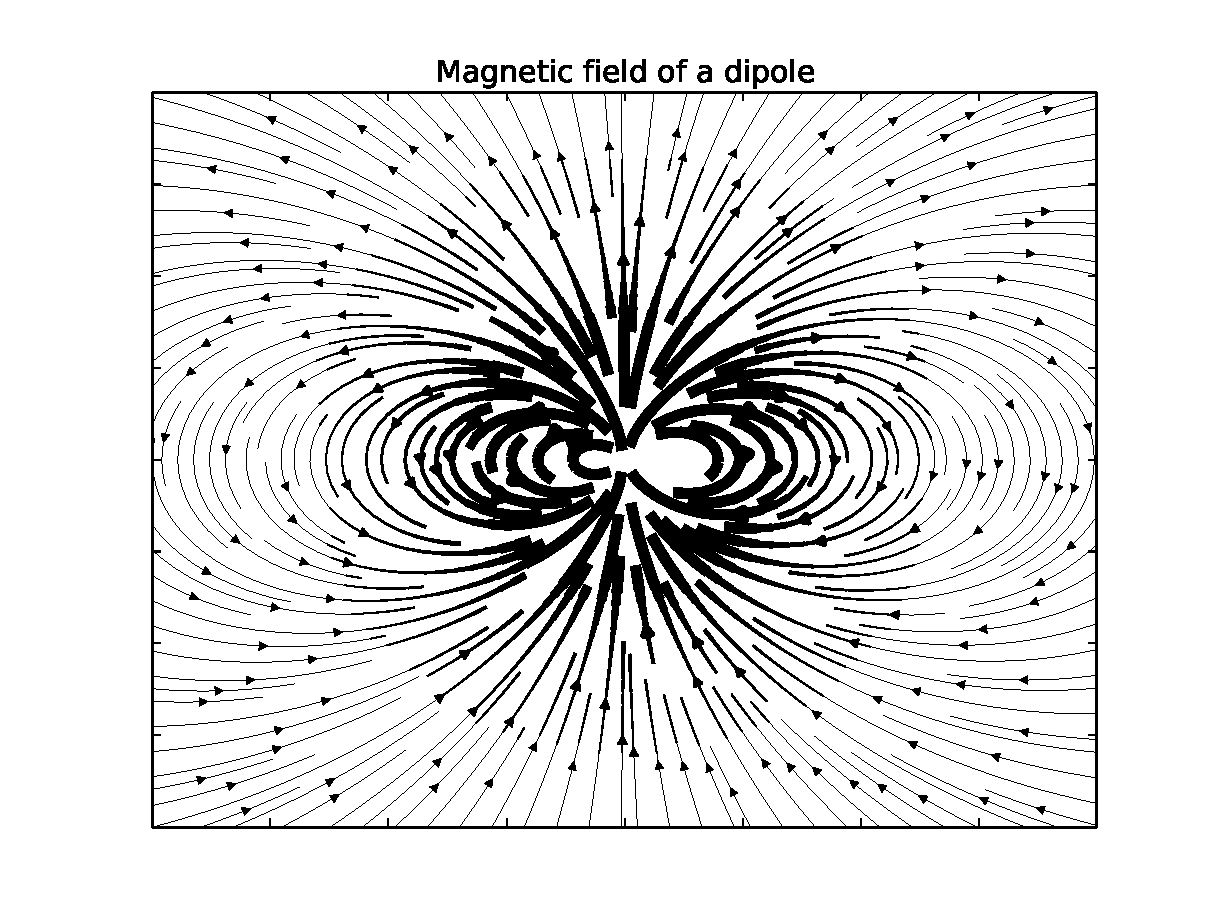
\includegraphics[width=0.8\textwidth]{Figures/dipole_field.pdf} 
\caption{The magnetic field generated by a single magnetic dipole located at the origin pointing in the $y$-direction. Broad field lines indicate a strong magnetic field.}
\label{fig:dipole_field} 
\end{center}
\end{figure}

In Figure \ref{fig:dipole_field} one can see that the demagnetizing field has a tendency to point in a different direction than the magnetization. At a position that is perpendicular to the magnetization the field is completely anti-aligned with the magnetization. Inserting \eqref{eq:demagfield} into \eqref{eq:demagenergy} one finds that the energy is

\begin{align}
\label{eq:demagenergy_mag}
E_D = \frac{\mu_0}{8\pi} \int \d {^3}r \int \d {^3}r' (\frac{\vec{M} (\vec{r}) \cdot \vec{M} (\vec{r'})}{|\vec{r}-\vec{r'}|^3} - \frac{3(\vec{M}(\vec{r}) \cdot (\vec{r}-\vec{r'})) (\vec{M}(\vec{r'}) \cdot(\vec{r}-\vec{r'}))}{|\vec{r}-\vec{r'}|^5}).
\end{align}

The energy is small when the total magnetization in the magnet is small, the demagnetizing field will therefore try to reduce the total magnetic moment in the magnet as discussed earlier. 

This integrand in \eqref{eq:demagenergy_mag} can be rewritten in a tensor form \cite{kruger2006current}. Using the relation

\begin{align}
\partial_i \frac{1}{|\vec{r}-\vec{r'}|} = -\frac{r_i-r_i'}{|\vec{r}-\vec{r'}|^3}
\end{align}

it is easy to see that

\begin{align*}
\partial_i\partial_j \frac{1}{|\vec{r}-\vec{r'}|} &= \partial_i(-\frac{r_j-r_j'}{|\vec{r}-\vec{r'}|^3}) \\
&= -\frac{\delta_{ij}}{|\vec{r}-\vec{r'}|^3}+3\frac{(r_i-r_i')(r_j-r_j')}{|\vec{r}-\vec{r'}|^5}.
\end{align*}

Defining the continuous demagnetization tensor to be

\begin{align}
N_{ij}(\vec{r}-\vec{r'}) = -\frac{1}{4\pi}\partial_i\partial_j \frac{1}{|\vec{r}-\vec{r'}|},
\end{align}

the demagnetization energy and field can then be written as

\begin{align}
E_D &= \frac{\mu_0}{2} \int \d {^3}r \int \d {^3}r' \vec{M}(\vec{r}) N(\vec{r}-\vec{r'})\vec{M}(\vec{r'}), \\
\vec{H}_D(\vec{r}) &= - \int \d {^3}r' N(\vec{r}-\vec{r'})\vec{M}(\vec{r'}).
\end{align}

Something worth noting is that if the demagnetization tensor $\bar{N}(\vec{r}-\vec{r'})$ is strictly diagonal, the energy can be written as

\begin{align}
E_D = \mu_0(N_{xx}M_x^2+N_{yy}M_y^2+N_{zz}M_z^2).
\end{align}

This is the case for ellipsoidal bodies \cite{kruger2006current}. This form of the demagnetization energy is similar to that of the uniaxial anisotropic energy in \eqref{eq:uniaxialanisotropy}. This means that ellipsoidal magnetic particles cause shape anisotropy, assuming the magnetic particle is not spherical ($N_{xx} = N_{yy} = N_{zz}$).

\subsection{Zeeman energy}
The Zeeman energy describes the energy from the interaction between the magnetization of the magnet and an external field $\vec{H}_{Z}$. The Zeeman energy is on the same form as the demagnetization energy in \eqref{eq:demagenergy}, with the internally generated demagnetization field replaced by the external magnetic field:

\begin{align}
\label{eq:zeemanenergy}
E_Z = -\mu_0\int \d {^3}r \vec{M}(\vec{r})\cdot\vec{H}_{Z}(\vec{r}).
\end{align}

The factor 1/2 in the demagnetization energy is to account for double counting of the dipole interactions, and is therefore not included in the Zeeman energy as the magnetic moments only interact with an external field. The Zeeman energy is at its minimum when the magnetization is aligned with the external field.

\subsection{Exchange energy}
Spins on a lattice will have an exchange energy with their nearest neighbors, as given by the Heisenberg Hamiltonian

\begin{align}
\label{eq:heisenberg}
H = -J\sum_{<i, j>} \vec{S}_i\cdot\vec{S}_j = -\frac{J S^2}{M_s^2}\sum_{<i, j>} \vec{M}_i\cdot\vec{M}_j,
\end{align}

with $J$ being the exchange integral. For a ferromagnet the lowest exchange energy is when the spins are aligned, meaning $J>0$. In the Hamiltonian we sum over each nearest neighbor pair $<i, j>$. To perform the sum we look at the magnetization in the continuum limit, with a slowly varying magnetization. It is then possible to do a Taylor expansion around the magnetization $\vec{M}_i$. If one only looks at a Taylor expansion in the $x$-direction, it can be written as

\begin{align}
\label{eq:taylormag}
\vec{M}_{i+1} \approx \vec{M}_i + a\frac{\partial \vec{M}_i}{\partial x} + \frac{a^2}{2}\frac{\partial^2 \vec{M}_i}{\partial^2 x},
\end{align}

with $a$ being the lattice constant and $\vec{M}_{i+1}$ the magnetization at the neighboring site to $\vec{M}_i$ along the $x$-axis. Similar expansions can be done in the $y$- and $z$-directions. Using this we can take a look at the contribution to the energy from $\vec{M}_i$ and its nearest neighbors in \eqref{eq:heisenberg}. For simplicity we consider a cubic lattice with a lattice constant $a$. Each lattice site has six nearest neighbors in three dimensions. Applying \eqref{eq:taylormag} to find the contributions to the energy from the nearest neighbors in the $x$-direction located at $\pm a \hat{x}$ relative to $\vec{M}_i$, we find

\begin{align*}
\vec{M}_i\cdot\vec{M}_{i-1}+\vec{M}_i\cdot\vec{M}_{i+1} &= 2\vec{M}_i\cdot\vec{M}_i + (a - a) \vec{M}_i\cdot\frac{\partial \vec{M_i}}{\partial x} + a^2\vec{M}_i\cdot\frac{\partial^2 \vec{M}_i}{\partial^2 x} \\
&= 2M_s^2 + a^2\vec{M}_i\cdot\frac{\partial^2 \vec{M}_i}{\partial^2 x}.
\end{align*}
Doing the same calculation for the nearest neighbors in the $y$- and $z$-directions we get that the exchange energy density from the magnetization at one site and its nearest neighbors is

\begin{align}
\epsilon_i = -\frac{JS^2}{a^3}(6+\frac{a^2}{M_s^2}\vec{M}_i\nabla^2\vec{M}_i).
\end{align}

To find the total exchange energy in the magnet we integrate the energy density over the volume of the magnet, so that

\begin{align}
\label{eq:exchangeenergylaplace}
E_E = -\int \d {^3}r \frac{JS^2}{2aM_s^2} \vec{M}(\vec{r})\nabla^2\vec{M}(\vec{r}).
\end{align}

The constant term in the energy has been ignored, and the factor $1/2$ has been introduced to account for the double counting of the interaction pairs. The energy in \eqref{eq:exchangeenergylaplace} can be rewritten to a more common form. Using that 

\begin{align}
\nabla(\vec{M} (\nabla\cdot\vec{M})) = (\nabla\cdot\vec{M})^2 + \vec{M}\nabla^2\vec{M},
\end{align}

and that

\begin{align}
\nabla M_s^2 = \nabla (\vec{M}\cdot\vec{M}) = 2\vec{M}(\nabla\cdot\vec{M}) = 0
\end{align} 

because $M_s$ is a constant, we find

\begin{align}
\vec{M}\nabla^2\vec{M} = - (\nabla\cdot\vec{M})^2.
\end{align}

This means that the energy in \eqref{eq:exchangeenergylaplace} becomes

\begin{align}
\label{eq:exchangeenergydiv}
E_E = \int \d {^3}r \frac{A}{M_s^2} (\nabla\cdot\vec{M}(\vec{r}))^2,
\end{align}

where we have introduced the exchange constant $A$. As one can see, the energy depends on the divergence of the magnetization squared, meaning the variation in the magnetization. Because the exchange constant $A$ is positive in a ferromagnet, the exchange energy is higher the more the magnetization varies. This can also easily be seen from \eqref{eq:heisenberg}, it costs energy when the spins are not aligned when $J>0$, which is the case in a ferromagnet. To minimize the exchange energy the magnetization therefore has to vary slowly. On short ranges this effect is much stronger than the demagnetization and magnetocrystalline anisotropy. This is why neighbouring spins have a tendency to align in a ferromagnet, while on longer ranges when the demagnetization effect becomes stronger than the exchange interaction the spins tend to be anti-aligned.

\section{Landau--Lifshitz--Gilbert equation}
The time evolution of the magnetization in a magnet is described by the Landau--Lifshitz--Gilbert (LLG) equation. To get an understanding of the origin of the equation, it is useful to look at the time evolution of spin, as the magnetic moment and therefore the magnetization is proportional to it. 

\subsection{Larmor precession}
The time evolution of an angular momentum $\vec{L}$ can be described by a variation on the classical Newton's second law for rotation:

\begin{align}
\label{eq:newton2rotation}
\frac{\textrm{d} \vec{L}}{\textrm{d} t} = \vec{T},
\end{align}

where $\vec{T}$ is the torque acting on the angular momentum. Spin is often compared to an intrinsic angular momentum of the electron, and will satisfy the same equation, with the exception that the vectors become operators as spin is a quantum mechanical effect. We are interested in looking at the magnetization on a microscopic scale, which would correspond to a semi-classical limit, so the quantum mechanical operators are replaced by their expectation values. 

A magnetic moment $\vec{\mu}$ will precess around an external magnetic field $\vec{H}$. This is known as Larmor precession, and is given by the torque

\begin{align}
\label{eq:larmortorque}
\vec{T} = \vec{\mu} \times \vec{H} = -\gamma \vec{S} \times \vec{H},
\end{align}

where we have introduced the gyromagnetic ratio $\gamma$. The gyromagnetic ratio gives the ratio of the magnetic moment relative to the spin of a particle. For the electron the gyromagnetic ratio is given by

\begin{align}
\gamma = \frac{g_e\mu_B}{\hbar},
\end{align}

with the $g$-factor $g_e \approx 2$ and $\mu_B$ being the Bohr magneton

\begin{align}
\mu_B = \frac{e\hbar}{2m_e}.
\end{align}

By inserting \eqref{eq:larmortorque} into \eqref{eq:newton2rotation} and replacing the angular momentum with spin, we get

\begin{align}
\frac{\textrm{d} \vec{S}}{\textrm{d} t} =- \gamma \vec{S} \times \vec{H},
\end{align}

or by replacing the spin with the magnetization using that $\vec{S}$ is proportional to $\vec{M}$:

\begin{align}
\label{eq:mag_undamped}
\frac{\textrm{d} \vec{M}}{\textrm{d} t} = -\gamma \vec{M} \times \vec{H}.
\end{align}

\subsection{Effective field}

If the magnetic moments were free, meaning they did not interact with each other, the field $\vec{H}$ in \eqref{eq:mag_undamped} would just be the magnetic field in the material. The magnetic field is the sum of any external field and the internal demagnetizing field discussed earlier. The magnetic moments are not free, however, as we have effects such as exchange interaction between the magnetic moments and magnetic anisotropy. Landau and Lifshitz introduced an effective field $\vec{H}_{eff}$ that replaced the magnetic field $\vec{H}$ in \eqref{eq:mag_undamped} that would minimize the energy in the system at equilibrium \cite{LandauLifshitz1935}. The terms in the micromagnetic energy discussed earlier were the anisotropic energy, demagnetization energy, the Zeeman energy and the exchange energy. Using the results derived earlier, we can write the total energy in the system as

\begin{align}
\label{eq:micromagneticenergy}
E(\vec{M}) = \int \d {^3} r (\epsilon_A(\vec{M}) + \epsilon_D(\vec{M}) + \epsilon_Z(\vec{M}) + \epsilon_E(\vec{M})),
\end{align}

where the $\epsilon$'s are the energy densities of the different terms. In equilibrium we must require that $\delta E=0$, with $\delta E$ being defined by

\begin{align}
\label{eq:deltaE}
\delta E = \int_a^b \frac{\delta E[\vec{M}]}{\delta \vec{M}(\vec{r})}\cdot \delta \vec{M}(\vec{r}) \d {\vec{r}}.
\end{align}

The functional derivative $\frac{\delta E[\vec{M}]}{\delta \vec{M}(\vec{r})}$ is just the left hand side of the Euler-Lagrange equation, so that

\begin{align}
\label{eq:functionaldiff}
\frac{\delta E[\vec{M}]}{\delta \vec{M}(\vec{r})} = \frac{\partial E[\vec{M}]}{\partial \vec{M}(\vec{r})} - \frac{\partial}{\partial x} \frac{\partial E[\vec{M}]}{\partial (\frac{\partial \vec{M}}{\partial x})} - \frac{\partial}{\partial y} \frac{\partial E[\vec{M}]}{\partial (\frac{\partial \vec{M}}{\partial y})} - \frac{\partial}{\partial z} \frac{\partial E[\vec{M}]}{\partial (\frac{\partial \vec{M}}{\partial z})}.
\end{align}

As $|\vec{M}| = M_s$ is a constant, $\delta \vec{M}$ must be perpendicular to $\vec{M}$. Because of this, $\frac{\delta E[\vec{M}]}{\delta \vec{M}(\vec{r})}$ must be parallel to $\vec{M}$ for $\delta E$ to be 0 for arbitrary choices of $a$ and $b$. In \eqref{eq:mag_undamped} one can see that the system is in equilibrium if the effective field $\vec{H}_{eff}$ is parallel to $\vec{M}$, therefore the effective field must also be parallel to $\frac{\delta E[\vec{M}]}{\delta \vec{M}(\vec{r})}$. It is reasonable to assume that one of the terms in the effective field will just be the external magnetic field $\vec{H}_Z$. We can therefore look at $\epsilon_Z$, the energy density in \eqref{eq:zeemanenergy}, to find the proportionality constant. It is easy to see that by letting

\begin{align}
\vec{H}_{eff} = -\frac{1}{\mu_0}\frac{\delta \epsilon[\vec{M}]}{\delta \vec{M}(\vec{r})},
\end{align}

one of the terms in the effective field will be the external field $\vec{H}_Z$ (with $\epsilon = \frac{\partial E}{\partial V}$). By using this definition and the definition of the functional derivative in \eqref{eq:functionaldiff}, one then finds that the effective field is

\begin{align}
\label{eq:effectivefield}
\vec{H}_{eff}(\vec{r}) = \vec{H}_Z(\vec{r}) + \vec{H}_D(\vec{r}) + \frac{2A}{\mu_0M_s^2}\nabla^2\vec{M}(\vec{r}) -\frac{1}{\mu_0}\frac{\delta \epsilon_A[\vec{M}]}{\delta \vec{M}(\vec{r})}.
\end{align}

The last term depends on what kind of anisotropy there is in the material. For a uniaxial anisotropy as in \eqref{eq:uniaxialanisotropy}, the effective field term becomes 

\begin{align}
\label{eq:effielduniaxialani}
-\frac{1}{\mu_0}\frac{\delta \epsilon_A[\vec{M}]}{\delta \vec{M}(\vec{r})} = -\frac{2K_1}{M_s^2}(\vec{M}(\vec{r})\cdot\hat{n})\hat{n} - \frac{4K_2}{M_s^4}(\vec{M}(\vec{r})\cdot\hat{n})^3\hat{n}
\end{align}

up to fourth order in the directional cosine. For a cubic anisotropy the energy density $\epsilon_A$ becomes the integrand in \eqref{eq:cubicanisotropy} instead.

Looking at the effective field in \eqref{eq:effectivefield} we see that it consists of the external magnetic field and the demagnetizing field, as one would expect, and two effective field terms that originate from quantum mechanical effects. The exchange interaction between the magnetic moments cause an effective field that points in the direction that is the average rate of change in the magnetization $\vec{M}(\vec{r})$ at a point $\vec{r}$. If the magnetization is uniform or varies very slowly in space, the effective field from the exchange interaction is very small or non-existent. If the magnetization varies at a significant rate, the effective field from the exchange interaction will point in a direction that will try to decrease this rate of change, thereby minimizing the exchange energy. If one studies the effective field from the anisotropic energy, one finds that the field will try to align the magnetization with the easy axis, or move the magnetization away from the hard axis, depending on the axes in the material. For a uniaxial anisotropy, the effective field is described by \eqref{eq:effielduniaxialani}. We discussed earlier that the direction $\hat{n}$ was parallel to the easy axis if the anisotropy constants $K_i$ were $<0$, and it was parallel to the hard axis if the anisotropy constants were $>0$. Considering the case of $\hat{n}$ being parallel to te easy axis first, we see that the effective field will point in the direction that the component of $\vec{M}(\vec{r})$ has along the easy axis. This is regardless of which of the two directions the component points in, as we only have odd powers of $(\vec{M}(\vec{r})\cdot\hat{n})$ in the field. If $\hat{n}$ is parallel to the hard axis, the constants $K_i$ are positive, and the field points in the opposite direction that the component of $\vec{M}(\vec{r})$ has along the hard axis. The effective field then tries to reduce the component along the hard axis, to minimize the anisotropic energy.

\subsection{Damping and the Landau--Lifshitz equation}
The time evolution in \eqref{eq:mag_undamped} only describes the precession of the magnetization around a field $\vec{H}$. This system is not in equilibrium unless the magnetization is parallel to the field. In a physical system the magnetization will eventually relax to equilibrium. To model this, Landau and Lifshitz introduced a damping term that is perpendicular to the magnetization and the direction of the precession around the field \cite{LandauLifshitz1935}. The damping term will point in a direction as to attempt to align the magnetization with the field, \eqref{eq:mag_undamped} therefore becomes

\begin{align}
\label{eq:LL}
\frac{\textrm{d} \vec{M}}{\textrm{d} t} = -\gamma (\vec{M} \times \vec{H}_{eff} + \frac{\alpha}{M_s} \vec{M}\times(\vec{M}\times\vec{H}_{eff})),
\end{align}

with $\alpha > 0$ being a dimensionless damping constant. This is known as the Landau--Lifshitz equation.

\subsection{The Gilbert damping term}
The Landau-Lifshitz equation agrees with experiments for low damping constants $\alpha$, but it does not perform well when the damping constants get large. To improve the model of damping in \eqref{eq:LL}, Gilbert proposed a damping term on a different form. By comparing the damping of the magnetization to dampings in other physical systems, Gilbert used a Rayleigh dissipation functional that depended on the time derivative of the magnetization to model the dissipative force \cite{Gilbert2004Classics}. This is analogous to a model for friction where the Rayleigh dissipation functional depends on the time derivative of the position, which is just the velocity. By using this new damping term that is a function of $\frac{\textrm{d} \vec{M}}{\textrm{d} t}$, the Gilbert form of the Landau--Lifshitz equation becomes

\begin{align}
\label{eq:LLG_implicit}
\frac{\textrm{d} \vec{M}}{\textrm{d} t} = -\gamma \vec{M} \times (\vec{H}_{eff} - \eta \frac{\textrm{d} \vec{M}}{\textrm{d} t}),
\end{align}

with $\eta$ being a damping parameter. This equation is implicit in $\frac{\textrm{d} \vec{M}}{\textrm{d} t}$. It can be shown that \eqref{eq:LLG_implicit} and \eqref{eq:LL} are mathematically equivalent by rewriting it to an explicit form in $\frac{\textrm{d} \vec{M}}{\textrm{d} t}$. To rewrite \eqref{eq:LLG_implicit} we must find an expression for $\vec{M}\times\frac{\textrm{d} \vec{M}}{\textrm{d} t}$ that does not involve a cross-product. To do this we can just take the cross product of \eqref{eq:LLG_implicit} with $\vec{M}$ from the left:

\begin{align}
\label{eq:mtimesdmdt}
\vec{M}\times\frac{\textrm{d} \vec{M}}{\textrm{d} t} = -\gamma \vec{M}\times(\vec{M}\times\vec{H}_{eff}) + \gamma\eta \vec{M}\times(\vec{M}\times\frac{\textrm{d} \vec{M}}{\textrm{d} t}).
\end{align}

The first term on the right hand side is proportional to one of the terms in \eqref{eq:LL}, so we leave that be. The triple cross product involving $\frac{\textrm{d} \vec{M}}{\textrm{d} t}$ can be rewritten using the relation $\vec{A}\times(\vec{B}\times\vec{C}) = (\vec{A}\cdot\vec{C})\vec{B} - (\vec{A}\cdot\vec{B})\vec{C}$:

\begin{align}
\label{eq:mag_triple_crossproduct}
\vec{M}\times(\vec{M}\times\frac{\textrm{d} \vec{M}}{\textrm{d} t}) =  (\vec{M}\cdot\frac{\textrm{d} \vec{M}}{\textrm{d} t})\vec{M} - (\vec{M}\cdot\vec{M})\frac{\textrm{d} \vec{M}}{\textrm{d} t}.
\end{align}

The first term on the right hand side can be found by taking the scalar product of $\vec{M}$ and \eqref{eq:LLG_implicit}. It is easy to see that this is 0, as the entire right hand side of \eqref{eq:LLG_implicit} is perpendicular to $\vec{M}$. It is also worth noting that when $\vec{M}\cdot \frac{\textrm{d} \vec{M}}{\textrm{d} t} = 0$ the modulus $|\vec{M}| = M_s$ is a constant, as 

\begin{align}
\frac{\textrm{d}}{\textrm{d} t} (M_s^2) = \frac{\textrm{d}}{\textrm{d} t} (\vec{M}\cdot\vec{M}) = 2 \vec{M} \cdot \frac{\textrm{d} \vec{M}}{\textrm{d} t}.
\end{align}

This is in agreement with what we have discussed earlier. The second term on the right hand side in \eqref{eq:mag_triple_crossproduct} is just $-M_s^2 \frac{\textrm{d} \vec{M}}{\textrm{d} t}$. Combining the results of \eqref{eq:mtimesdmdt} and \eqref{eq:mag_triple_crossproduct} and inserting it into \eqref{eq:LLG_implicit}, we can simplify the expression to

\begin{align}
\label{eq:LLG_oldparam}
\frac{\textrm{d} \vec{M}}{\textrm{d} t} = -\frac{\gamma}{1 + \gamma^2\eta^2 M_s^2}(\vec{M}\times\vec{H}_{eff} + \gamma\eta \vec{M} \times (\vec{M}\times\vec{H}_{eff})).
\end{align}

Comparing this to the Landau--Lifshitz equation in \eqref{eq:LL} we see that by letting

\begin{align}
\eta &= \frac{\alpha}{\gamma M_s}, \\
\tilde{\gamma} &= \frac{\gamma}{1+\alpha^2},
\end{align}

\eqref{eq:LLG_oldparam} can be written on the form of the Landau--Lifshitz equation:

\begin{align}
\label{eq:LLG}
\frac{\textrm{d} \vec{M}}{\textrm{d} t} = -\tilde{\gamma} (\vec{M} \times \vec{H}_{eff} + \frac{\alpha}{M_s} \vec{M}\times(\vec{M}\times\vec{H}_{eff})).
\end{align}

This is the explicit Landau--Lifshitz--Gilbert equation. The difference between the Landau--Lifshitz and the Landau--Lifshitz--Gilbert equation is that the gyromagnetic ratio in the LLG equation is redefined to include the dimensionless damping parameter $\alpha$. When $\alpha \ll 1$, the Landau--Lifshitz equation is a good approximation of the LLG equation, but as the damping parameter becomes larger the correction in the gyromagnetic ratio becomes significant. The LLG equation agrees better with experiments where the damping constant $\alpha$ is large \cite{GilbertKelly1955}.

\section{Domain walls}

\section{Domain wall dynamics}

\section{Skyrmions}

\section{References}
\bibliography{main}
\bibliographystyle{unsrt}


\end{document}